
Computing the diameter of an input (undirected, unweighted) graph $G$ is a classic computational 
problem that can be trivially solved in $\Oh(nm)$ time\footnote{We follow the convention that the vertex and the edge count of the input graph are denoted by $n$ and $m$, respectively.}.
In 2013, Roditty and Vassilevska-Williams showed that this running
time bound cannot be significantly improved in general:
any algorithm distinguishing graphs of diameter $2$ and $3$
running in time $\Oh(m^{2-\varepsilon})$, for any fixed $\varepsilon > 0$,
would break the Strong Exponential Time Hypothesis~\cite{RodittyW13}. 
This motivates the search for restrictions on $G$ that would make the  problem of computing the diameter more tractable.

As shown by Cabello and Knauer~\cite{CabelloK09}, sophisticated orthogonal range query data structures allow near-linear diameter
computation in graphs of constant treewidth.
A breakthrough result by Cabello~\cite{Cabello19} showed that 
the diameter of an $n$-vertex planar graph can be computed in $\widetilde{\Oh}(n^{11/6})$ time;
this complexity has been later improved by Gawrychowski, Kaplan, Mozes, Sharir, and Weimann to
$\widetilde{\Oh}(n^{5/3})$~\cite{GawrychowskiKMS21}\footnote{The $\widetilde{\Oh}(\cdot)$ notation hides factors polylogarithmic in $n$, and the $\Oh_k(\cdot)$ notation hides factors depending on a parameter $k$.}.
A subsequent line of research~\cite{DucoffeHV22,DurajKP23,LeW24}
generalized this result to $K_h$-minor-free graphs:
for every integer $h$, there exists a constant $c_h > 0$ such that the diameter
problem in $n$-vertex $K_h$-minor-free graphs can be solved in time $\Oh_h(n^{2-c_h})$. 
In the works~\cite{DurajKP23,LeW24}, it holds that $c_h = \Omega\left(\frac{1}{h}\right)$; so the savings tend to zero as the size of the excluded clique minor increases.

However, known lower bounds, including the one of~\cite{RodittyW13}, does not exclude the possibility
that $c_h$ can be made a universal constant. That is, no known lower bound refutes
the following conjecture:
\begin{conjecture}\label{conj:taunt}
There exists a constant $c > 0$ such that,
for every integer $h > 1$, the diameter problem in (unweighted, undirected) $n$-vertex
$K_h$-minor-free graphs can be solved in time $\Oh_h(n^{2-c})$. 
\end{conjecture}

\paragraph{Graphs of bounded Euler genus.}
Our main result is the verification of \Cref{conj:taunt} for graphs
of bounded Euler genus. Furthermore, our algorithm computes also the eccentricies
of all the vertices of the input graph $G$. Recall here that
    the eccentricity of a vertex $v \in V(G)$ is defined as
    $\ecc(v) \coloneqq \max_{u \in V(G)} \dist_G(u,v)$, where $\dist_G(\cdot,\cdot)$ is the distance metric in $G$.
\begin{theorem}\label{thm:main-genus}
For every integers $k \geq 1$,
there exists an algorithm that, given an (unweighted, undirected) $n$-vertex graph $G$
of Euler genus at most $k$, runs in time $\Oh_k(n^{2-\frac{1}{25}})$
and computes the diameter of $G$ and the eccentricity of every vertex of $G$.
\end{theorem}

We remark that in~\cite[Section~9]{Cabello19}, Cabello briefly speculated that his approach could be also generalized to graphs embeddable on surfaces of bounded genus. However, as noted in \cite{Cabello19}, this would require significant effort, as the technique works closely on the embedding and in surfaces of higher genus, additional topological hurdles arise. In contrast, in our proof of \Cref{thm:main-genus} the main ingredient is an improved combinatorial bound on the number of so-called \emph{distance profiles}~\cite{LeW24} in graphs of bounded Euler genus. This proof uses topology only very lightly, while the rest of the argument is rather standard and topology-free. All in all, we obtain a robust methodology of approaching the problem, which, as we will see, can be also used to attack \Cref{conj:taunt} to some extent.

To explain our bound on distance profiles, we need to recall several relevant definitions.

Let $G$ be a graph, $R \subseteq V(G)$ be a subset of vertices, and $s_R \in R$ be a vertex in $R$.
The \emph{distance profile} of a vertex $u \in V(G)$ to $R$ (relative to $s_R$)
  is the function $\distprofile{R}{s_R}{u} \colon R \to \mathbb{Z}$ defined as follows:
  \[ \distprofile{R}{s_R}{u}(s) = \dist_G(u,s) - \dist_G(u,s_R)\qquad \textrm{for all }s\in R. \]
Note that provided $R$ is connected\footnote{A subset of vertices $R$ of a graph $G$ is {\em{connected}} if the induced subgraph $G[R]$ is connected.}, we have
$\distprofile{R}{s_R}{u}(s) \in \{-|R|,-|R|+1,\ldots,|R|-1,|R|\}$. In~\cite{LeW24},
Le and Wulff-Nilsen proved that if $R$ is connected and $G$ is $K_h$-minor-free, then
the set system $$\left\{ \left\{(s,i) \in R \times \{-|R|,\ldots,|R|\}~|~i \leq \distprofile{R}{s_R}{u}(s)\right\}~\colon~u \in V(G)\right\}$$ has VC dimension at most $h-1$. Hence, by applying the Sauer-Shelah Lemma we obtain that
\begin{theorem}[\cite{LeW24}]\label{thm:distprofiles-LeW24}
For every integer $h\geq 1$, $K_h$-minor-free graph $G$, connected set $R \subseteq V(G)$, and  $s_R \in R$, there are at most $\Oh_h(|R|^{2h-2})$
different distance profiles to $R$ relative to $s_R$. 
\end{theorem}
The VC dimension argument applied above inevitably leads to a bound with the exponent depending on $h$.
We show that for  graphs of bounded Euler genus, the bound of \Cref{thm:distprofiles-LeW24}
can be improved to a polynomial of degree independent of the parameter.
\begin{theorem}\label{thm:distprofiles}
For every integer $k\geq 1$, (unweighted, undirected) graph $G$ of Euler genus at most~$k$, connected set $R \subseteq V(G)$, and $s_R \in R$,
the number of distance profiles to $R$ relative to $s_R$
is at most~$\Oh_k(|R|^{12})$.
\end{theorem}
The main idea behind the proof of \Cref{thm:distprofiles} is the following simple
observation:
if $P$ is a shortest path from some $u \in V(G)$ to $s_R$, then, as one walks along $P$
from $u$ to $s_R$, the distance profile of the current vertex to $R$ can only (point-wise) increase.
A slightly more technical modification of this argument works for shortest paths
from $u \in V(G)$ to $R$. This allows us to reduce the case of bounded Euler genus graphs
to the planar case by cutting along a constant number of shortest-to-$R$ paths,
and analysing how the distance profiles change during such a process.

One could ask whether an improvement similar to that of \Cref{thm:distprofiles}
would be possible even in the generality of $K_h$-minor-free graphs.
Unfortunately, it seems that \Cref{thm:distprofiles} is the limit of such improvements. More precisely, the following simple example shows that the linear dependency on $h$ in the exponent of the bound on the number of profiles is inevitable even in graphs of treewidth $h$ (which are  $K_{(h+1)^2}$-minor-free).


Let $0 < k \ll \ell$ be positive integers.
Let $R$ be a path of length $\ell$ and $v_1,\ldots,v_k$ be $k$ equidistant
points on $R$ (i.e., the distance between $v_i$ and $v_{i+1}$ is at least $p \coloneqq \lfloor \ell/(k-1) \rfloor$).
For every vector $\mathbf{a} = (a_1,\ldots,a_k) \in \{\ell, \ldots, \ell + p \}^k$,
construct a vertex $u(\mathbf{a})$ and, for every $i\in \{1,\ldots,k\}$, connect it with
$v_i$ using a path of length $a_i$.
This finishes the construction of the graph $G$; see~\Cref{fig:example} for an illustration.
Note that $G$ has treewidth at most $k+1$, because $G-\{v_1,\ldots,v_k\}$ is a forest.
Furthermore, since the distance between consecutive vertices $v_i$ is at least $p$, we have that
  $\dist_G(u(\mathbf{a}), v_i) = a_i$ for every vector $\mathbf{a}$ and $i\in \{1,\ldots,k\}$.
Consequently, if we restrict to vectors $\mathbf{a}$ with $a_1 = \ell$, 
every vertex $u(\mathbf{a})$ has a different distance profile to $R$ relative to $v_1$.
Finally, note that there are $(p + 1)^{k-1} \geq (\ell/(k-1))^{k-1} = \Omega_k(\ell^k)$ different
vectors $\mathbf{a}$ with $a_1=\ell$, giving that many different~profiles.
\begin{figure}[ht]
  \centering
  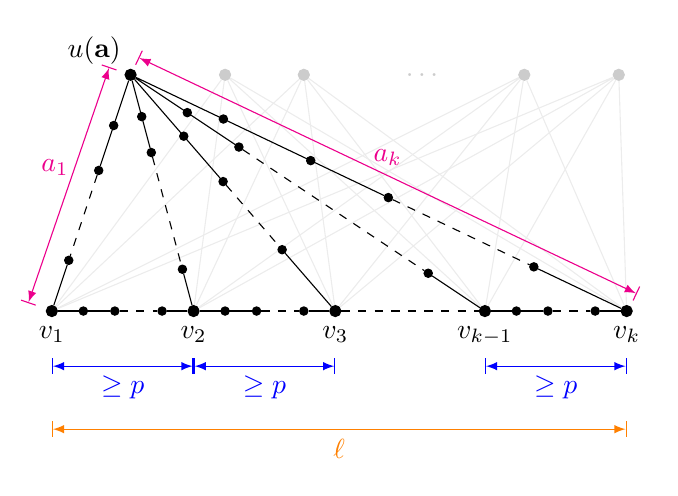
\begin{tikzpicture}
    \tikzset{black node/.style={draw, circle, fill = black, minimum size = 4pt, inner sep = 0pt}}
    \tikzset{small black node/.style={draw, circle, fill = black, minimum size = 3pt, inner sep = 0pt}}

    \node[black node, label={below:$v_1$}] (A) at (0,0) {};
    \node[black node, label={below:$v_2$}] (B) at (1.8,0) {};
    \node[black node, label={below:$v_3$}] (C) at (3.6,0) {};
    \node[black node, label={below:$v_{k-1}$}] (D) at (5.5,0) {};
    \node[black node, label={below:$v_k$}] (E) at (7.3,0) {};

  
    \node[small black node] at (0.4,0) {};
    \node[small black node] (Al) at (0.8,0) {};
    \node[small black node] (Ar) at (1.4,0) {};

    \node[small black node] at (2.2,0) {};
    \node[small black node] (Bl) at (2.6,0) {};
    \node[small black node] (Br) at (3.2,0) {};

    \node[small black node] at (5.9,0) {};
    \node[small black node] (Dl) at (6.3,0) {};
    \node[small black node] (Dr) at (6.9,0) {};


    \draw (A) -- (Al) (Ar) -- (B)
          (B) -- (Bl) (Br) -- (C)      
          (D) -- (Dl) (Dr) -- (E);
    \draw[dashed] (Al) -- (Ar) (Bl) --  (Br) (C) -- (D) (Dl) -- (Dr);

    \draw[blue] (0,-7mm) coordinate (S) edge[|<->|, >= latex] node[below]{\textcolor{blue}{$\ge p$}} (1.8,-7mm);
    \draw[blue] (1.8,-7mm) coordinate (S) edge[|<->|, >= latex] node[below]{\textcolor{blue}{$\ge p$}} (3.6,-7mm);
    \draw[blue] (5.5,-7mm) coordinate (S) edge[|<->|, >= latex] node[below]{\textcolor{blue}{$\ge p$}} (7.3,-7mm);
    \draw[orange] (0,-15mm) coordinate (S) edge[|<->|, >= latex] node[below]{\textcolor{orange}{$\ell$}} (7.3,-15mm);

    \node[black node, label={[label distance=-2pt]120:$u(\mathbf{a})$}] (X) at (1,3) {};
    
    \node[black node,gray!40!white] (T) at (2.2,3) {};
    \node[black node,gray!40!white] (P) at (3.2,3) {};
    \node[black node,gray!40!white] (Q) at (6,3) {};
    \node[black node,gray!40!white] (R) at (7.2,3) {};
    \node[label={center:\textcolor{gray!40!white}{$\dots$}}] at (4.7,3) {};
    \draw[gray!15!white] (T) -- (A) (T) -- (B) (T) -- (C) (T) -- (D) (T) -- (E);
    \draw[gray!15!white] (P) -- (A) (P) -- (B) (P) -- (C) (P) -- (D) (P) -- (E);
    \draw[gray!15!white] (Q) -- (A) (Q) -- (B) (Q) -- (C) (Q) -- (D) (Q) -- (E);
    \draw[gray!15!white] (R) -- (A) (R) -- (B) (R) -- (C) (R) -- (D) (R) -- (E);

    \path (X) to node[small black node] [pos=0.2] {}  node[small black node] [pos=0.4] (X1) {} 
    node[small black node] [pos=0.8] (X2) {}(A);
    \path (X) to node[small black node] [pos=0.16] {}  node[small black node] [pos=0.32] (Y1) {} 
    node[small black node] [pos=0.84] (Y2) {}(B);
    \path (X) to node[small black node] [pos=0.25] {}  node[small black node] [pos=0.45] (Z1) {} 
    node[small black node] [pos=0.75] (Z2) {}(C);
    \path (X) to node[small black node] [pos=0.15] {}  node[small black node] [pos=0.3] (W1) {} 
    node[small black node] [pos=0.85] (W2) {}(D);
    \path (X) to node[small black node] [pos=0.18] {} node[small black node] [pos=0.36] {}  node[small black node] [pos=0.52] (V1) {} 
    node[small black node] [pos=0.82] (V2) {}(E);

    \draw (X) -- (X1) (X2) -- (A)
    (X) -- (Y1) (Y2) -- (B)
    (X) -- (Z1) (Z2) -- (C)
    (X) -- (W1) (W2) -- (D)
    (X) -- (V1) (V2) -- (E);
    \draw[dashed] (X1) -- (X2)  (Y1) -- (Y2) (Z1) -- (Z2) (W1) -- (W2) (V1) -- (V2);

    \draw[magenta] (0.73,3.1) coordinate edge[|<->|, >= latex] node[above]{\textcolor{magenta}{$a_1$~~~}} (-0.3,0.1);
    \draw[magenta] (1.1,3.22) coordinate edge[|<->|, >= latex] node[above]{\textcolor{magenta}{$a_k$}} (7.43,0.22);


  \end{tikzpicture}
  \caption{Illustration of a construction that shows that linear dependency on $h$ in the exponent of the bound on the number of profiles is inevitable, even in graphs of treewidth $h$.}
  \label{fig:example}
\end{figure}

Our algorithm for \Cref{thm:main-genus} follows closely the approach of Le and Wulff-Nilsen~\cite{LeW24} augmented by the bound provided by \Cref{thm:distprofiles}. Namely, we first compute an $r$-division of the input graph $G$
into regions of size $r=n^{\delta}$, for some small $\delta > 0$. Then we use \Cref{thm:distprofiles}
for individual regions $R$ to speed up the computation of distances between $R$ and $V(G) \setminus R$,
by grouping vertices outside $R$ according to their distance profiles 
to $R$. Each group is batch-processed in a single step.


\paragraph{Generalizations.}
Further, we show that our techniques combine well with the techniques for bounded
treewidth graphs of Cabello and Knauer~\cite{CabelloK09}.
First, we show that \Cref{conj:taunt} holds for classes of graphs
of bounded Euler genus with a constant number of \emph{apices}, i.e., vertices that are arbitrarily connected to the rest of the graph.

\begin{theorem}\label{thm:main-apices}
For every integers $g,k \geq 1$, 
there exists an algorithm that, given an (unweighted, undirected) $n$-vertex graph $G$
and a set $A \subseteq V(G)$ such that $|A| \leq k$ and $G-A$ is
of Euler genus at most $g$, runs in time $\Oh_{g,k}(n^{2-\frac{1}{25}} \log^{k-1} n)$
and computes the diameter of $G$ and the eccentricity of every vertex of $G$.
\end{theorem}
Second, we show that \Cref{conj:taunt} holds for classes of graphs
constructed by clique-sums of graphs as in \Cref{thm:main-apices}.
To state this result formally, we need some definitions. For a graph $G$,
   a \emph{tree decompostion} of $G$ is a pair $(T,\beta)$ where $T$ is a tree
  and $\beta$ is a function that assigns to every $t \in V(T)$ a \emph{bag} 
  $\beta(t) \subseteq V(G)$ such that (1) for every $v \in V(G)$, the set $\{t \in V(T)~|~v \in \beta(t)\}$ is nonempty and connected in $T$, and (2) for every $uv \in E(G)$ there exists $t \in V(T)$ with $u,v \in \beta(t)$. 
 The \emph{torso} of the bag $\beta(t)$ is constructed from $G[\beta(t)]$ by adding, for every
 neighbor $s$ of $t$ in $T$, all edges between the vertices of $\beta(s) \cap \beta(t)$.
\begin{theorem}\label{thm:main-decomp}
For every integer $k \geq 1$, 
there exists an algorithm with the following specification.
The input consists of an (unweighted, undirected) $n$-vertex graph $G$
together with a tree decomposition $(T,\beta)$ of $G$ and a set $A(t) \subseteq \beta(t)$ for
every $t \in V(T)$ satisfying the following properties:
\begin{itemize}[nosep]
\item For every node $t \in V(T)$, we have that $|A(t)| \leq k$ and the torso of $\beta(t)$ with the vertices
of $A(t)$ deleted is a graph of Euler genus at most $k$.
\item For every edge $st \in E(T)$, we have $|\beta(s) \cap \beta(t)| \leq k$.
\end{itemize}
The algorithm runs in time $\Oh_k(n^{2-\frac{1}{356}} \log^{6k} n)$ and computes
the diameter of $G$ and the eccentricity of every vertex of $G$.
\end{theorem}
Note that the statements of
\Cref{thm:main-apices,thm:main-decomp} require the set $A$ and
the decomposition $(T,\beta)$, respectively, to be provided explicitly on input;
this should be compared with more general statements where the algorithm is 
given only $G$ with a promise that such set $A$ or decomposition $(T,\beta)$ exist. At this point, we are not aware of any existing algorithm that would find in subquadratic time a set $A$ as in \Cref{thm:main-apices},
or the decomposition $(T,\beta)$ with the sets $A$ as in \Cref{thm:main-decomp}, even in the approximate sense. However, we were informed by Korhonen, Pilipczuk, Stamoulis, and Thilikos~\cite{KorhonenPST24priv} that it seems likely that the techniques introduced in the recent almost linear-time algorithm for minor-testing~\cite{KorhonenPS24} could be used to construct such an algorithm, with almost linear time complexity. With this result in place, the assumption about the decomposition and/or apex sets being provided on input could be lifted in \Cref{thm:main-apices,thm:main-decomp}; this is, however, left to future work.


\paragraph{Discussion.}
As one of the main outcomes of their theory of graph minors, Robertson and Seymour proved the following Structure Theorem~\cite{RobertsonS03a}: every $K_h$-minor-free graph $G$
admits a tree decomposition $(T,\beta)$ such that
\begin{itemize}[nosep]
 \item for every pair $s,t$ of adjacent nodes of $T$, the set $\beta(t) \cap \beta(s)$ has size $\Oh_h(1)$; and
 \item the torso of every bag $\beta(t)$ is ``nearly embedable'' into a surface of bounded (in terms of $h$) Euler~genus.
\end{itemize}
The notion of being ``nearly embeddable'' encompasses adding a constant number of apices (which can be handled by \Cref{thm:main-decomp}) and a constant number of so-called
vortices (which are not handled by \Cref{thm:main-decomp}). Thus, our methods fall short of verifying  \Cref{conj:taunt} in full generality due to vortices.

We remark that recently, Thilikos and Wiederrecht~\cite{ThilikosW22} proved a variant of the Structure Theorem, where under the stronger assumption of excluding a minor of a {\em{shallow vortex grid}}, instead of a clique minor, they gave a decomposition as above, but with torsos devoid of vortices. Thus, the decomposition for shallow-vortex-grid-minor-free graphs provided by~\cite{ThilikosW22} can be directly plugged into \Cref{thm:main-decomp}, with the caveat that~\cite{ThilikosW22} does not provide a subquadratic algorithm to compute the decomposition.

Coming back to \Cref{conj:taunt},
the simplest case
that we are currently unable to solve is the setting when the input is a planar graph plus a single vortex. More formally, for a fixed integer $k$, let $\mathcal{G}_k$ be the class of graphs
defined as follows. We have $G \in \mathcal{G}_k$ if there exist two subgraphs $G_0,G_1$
of $G$ and a sequence of vertices $v_1,\ldots,v_b$ in $V(G_0) \cap V(G_1)$
such that:
\begin{itemize}[nosep]
 \item $V(G) = V(G_0) \cup V(G_1)$,
 \item $E(G) = E(G_0) \cup E(G_1)$,
 \item $G_0$ admits a planar embedding where the vertices $v_1,\ldots,v_b$ lie on one face in
this order, and
\item $G_1$ admits a tree decomposition $(T_1,\beta_1)$, where $T_1$ is a path on nodes $t_1,\ldots,t_b$ and for every $i\in\{1,\ldots,b\}$, the bag $\beta_1(t_i)$ contains $v_i$
and is of size at most $k$.
\end{itemize}
It is easy to see that graphs from $\mathcal{G}_k$ are $K_{k+\Oh(1)}$-minor-free.
Do they satisfy \Cref{conj:taunt}? That is, is there a constant
$c > 0$ such that the diameter problem in $\mathcal{G}_k$ can be solved in
time $\Oh_k(n^{2-c})$?

\paragraph{Organization.}
We prove \Cref{thm:distprofiles} in \Cref{sec:distprofiles}.
\Cref{thm:main-apices} is proven in \Cref{sec:algo-genus}; note that \Cref{thm:main-genus} follows from \Cref{thm:main-apices}
for $k=1$. 
\Cref{thm:main-decomp} is proven in \Cref{sec:algo}.

